% !TEX root = Projektdokumentation.tex

\newglossaryentry{Usability-Tests}{name={Usability-Tests},description={Probanden aus der Zielgruppe der Anwendung werden Aufgaben gestellt, welche sie mit der bestehenden Anwendung lösen sollen. Dabei wird untersucht, welcher Weg zur Lösung der Aufgabe eingeschlagen wird und wo dabei Probleme auftauchen.}}

\newacronym{CN1}{CN1}{Computernetze 1}

\newglossaryentry{Wireframes}{name={Wireframes},description={Die Visualisierung stellt die Seitenstruktur und Featureumsetzung sehr grob und schematisch dar. Der Wireframe wird in schwarz-weiss-grau angefertigt und gleicht dadurch einer Skizze oder Bleistiftzeichnung. Dieses Art der Visualisierung ist sehr schnell, einfach und günstig zu erstellen. Dazu genügt Papier und Bleistift oder eine entsprechende Wireframe-Software.}}

\newacronym{UI}{UI}{User Interface}

\newglossaryentry{User Interface}{name={User Interface},description={Unter einer Benutzeroberfläche oder Benutzerschnittstelle (UI) versteht man die Art und Weise, wie Befehle und Daten in den Computer eingegeben werden. Die Benutzeroberfläche ist die Schnittstelle zwischen Computer und Mensch. \cite{itWissen_benutzeroberflache}}}

%Qualitätsmanagement: Messungen, Tests, Usability Tests, Code Review usw. (mit vollständiger Beschreibung der Anordnungen und Rahmenbedingungen)

\section{Usability}
Im Internet gibt es zahlreiche Online-Quizzes, auch für das schulische Umfeld. Damit Mobile Quiz häufig und gerne genutzt wird, gibt es einige Faktoren zu beachten. \cite{marketingfire.de} Dazu zählen unter anderem das Design und die Strukturierung der Seite. \\

Wie gut die bestehende Mobile Quiz - Version in diesen Bereichen abschneidet, kann mit einem \gls{Usability-Tests} festgestellt werden. Davon wurden zwei Durchführungen gemacht, wobei die erste zu Beginn der Arbeit dabei half, Schwierigkeiten in der Bedienung offenzulegen. Anschliessend flossen die Ergebnisse draus in die Aufgabenstellung mit ein. Gegen Ende der Arbeit fand dann die zweite Durchführung statt, um zu messen, welche Fortschritte durch die Arbeit gelungen sind.

\subsection{Methoden}
Bei den \gls{Usability-Tests} zu Beginn der Arbeit nahmen drei Studenten der \acrfull{CN1}-Vorlesung, ein Student aus der Raumplanung sowie ein Student aus dem 5. Semester Informatik teil, was der Zielgruppe von Mobile Quiz entspricht. Zudem hatten die Studenten aus \acrshort{CN1} erst wenig Erfahrung damit gesammelt. \\
Bei der Durchführung wurden die Teilnehmern in Situationen hineinversetzt, welche bei der Benutzung von Mobile Quiz oft vorkommen (siehe Usability-Test\_Aufgabenstellung). Die Teilnehmer wurden dabei eins zu eins beobachtet und Schwierigkeiten oder Abweichungen von den Erwartungen (siehe Usability-Test\_Erwartungen) notiert. Die Gesamtauswertung wurde anschliessend in einem separaten Dokument festgehalten (siehe Usability-Test\_Auswertung). Die erwähnten Dokumente befinden sich im Anhang.

\subsection{Erkenntnisse}
% Hier folgen sämtliche Erkenntnisse zum Bereich Usability.
% Auch die Auswertung was neu gemacht wird, kommt hier hin bzw. sicher eine Zusammenfassung und ganzes ist dann im Anhang.
Die Durchführung der \gls{Usability-Tests} zeigte, dass vor allem im Bereich der Benutzerführung Probleme vorhanden sind, denn die vorhandenen Funktionen werden nicht auf den ersten Blick gefunden.
Aus den Erkenntnissen der \gls{Usability-Tests} sowie den eigenen Tests mit dem MobileQuiz wurden die ersten \gls{Wireframes} erstellt, diese befinden sich im Anhang. 

\section{Codestatistik}
Mit Codestatistiken soll erkannt werden, ob sich die Codequalität während der Arbeit verbessert oder nicht. Dafür wird das Webtool Code Climate eingesetzt.

Der nachfolgende Screenshot zeigt den Stand der Codequalität ganz zu beginn des Projektes. Die bereits eingezeichneten Verbesserungen sind entstanden, da die Grundeinstellungen auf unsere Bedürfnisse angepasst und verfeinert wurden.

\begin{figure}[H]
	\centering
	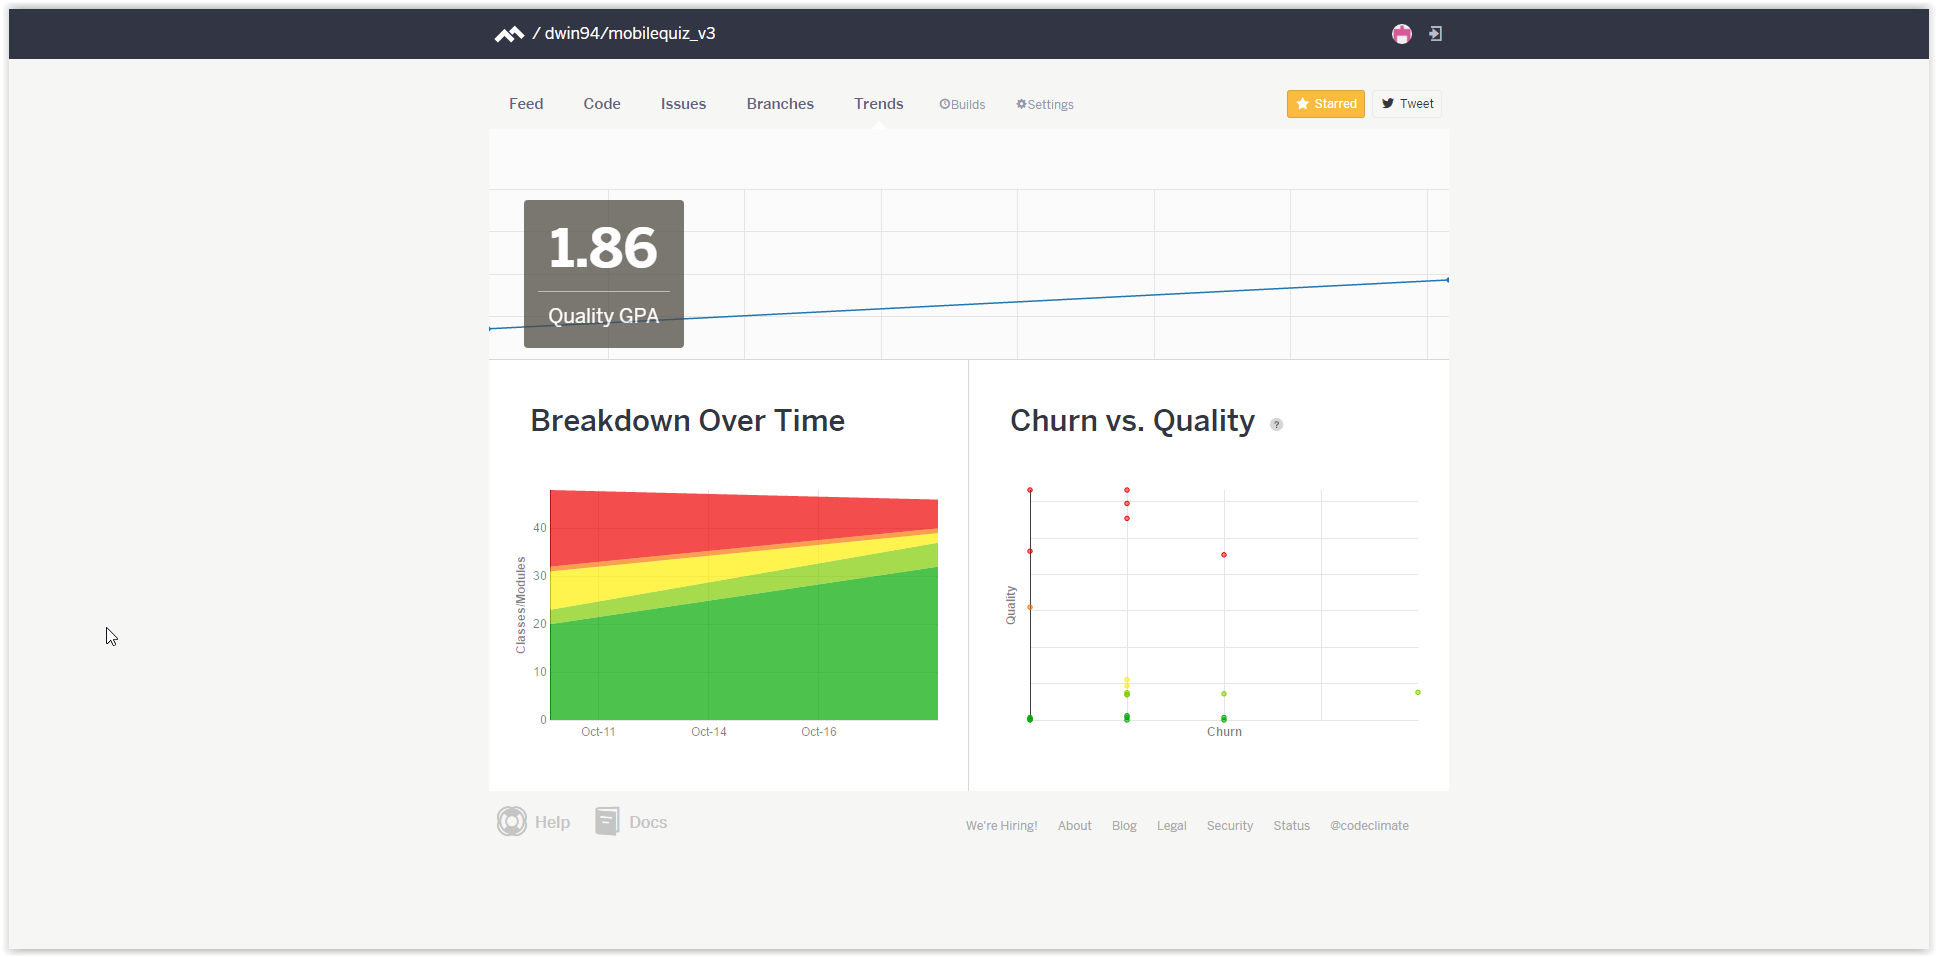
\includegraphics[width=1\textwidth
	]{Images/Stand_Beginn_181016.PNG}
	\caption{Code Climate Stand 18.10.2016 - nach der Verfeinerung der Regeln}
\end{figure}


\section{Systemtests mit Selenium}
%automatisierte Systemtests mit Selenium
Selenium IDE ist ein Firefox AddOn für Web-\acrfull{UI}-Tests. Es ermöglicht das Aufnehmen, die Bearbeitung, das Debuggen und das Abspielen von Tests. 

Mit der Hilfe dieses Tools können einfach \gls{User Interface} Tests durchgeführt werden.

\subsection{Methoden}
%Konkretes Vorgehen beschreiben
Mit dem Firefox Plugin von Selenium können die Abläufe die getestet werden sollen einfach aufgenommen werden. Das heisst der Benutzer spielt den korrekten Ablauf durch. Das einzige was von Hand gemacht werden muss, ist das assert-Statement, also die Prüfung, ob der Test korrekt durchgelaufen ist.

Alle erfassten Tests werden abgespeichert und können danach einfach abgespielt werden.

\subsection{Erkenntnisse}
%Was haben wir mit Hilfe von (siehe Titel) herausgefunden und wie werden wir es verbessern?
%Folgen sobald das Tool konkret eingesetzt wurde

\section{Code Review}
%Code Review mit GitHub Branch
%Einleitung
Mit einem Code Review wird die Codequalität sichergestellt. Dabei schaut sich jeweils derjenige, welcher den Code nicht geschrieben, den Code des anderen an. 


\subsection{Methoden}
%Konkretes Vorgehen beschreiben
Die Code Reviews wurden mit Github Branches gemacht. Das heisst der Entwickler eröffnet für seine neuen Features ein Github Branch und bevor dieser wieder in den Master merged werden kann, schaut sich das andere Teammitglied den Branch an und gibt in frei.

\subsection{Erkenntnisse}
%Was haben wir mit Hilfe von (siehe Titel) herausgefunden und wie werden wir es verbessern?
%Folgen sobald konkret eingesetzt wurde

\section{Unit-Tests}
%Unit-Tests mit PHPUnit
%Einleitung
Die Unit-Tests sind dazu da, einzelne Funktionen zu testen. Wenn eine Basis von Unit-Test bestehen, welche die Funktionalität des Codes abdecken, kann gut Refactoring betrieben werden. 

\subsection{Methoden}
%Konkretes Vorgehen beschreiben
Das Testen wurde mit PHPUnit umgesetzt. Diese Test werden bei jedem commit automatisch vom Continuous Integration Server, in unserem Fall Travis CI, ausgeführt. So wird bei jedem commit geschaut, ob noch alles funktioniert

\subsection{Erkenntnisse}
%Was haben wir mit Hilfe von (siehe Titel) herausgefunden und wie werden wir es verbessern?
%Folgen sobald konkret eingesetzt wurde



